%
% amplitudenmodulation.tex
%
% (c) 2020 Prof Dr Andreas Müller, Hochschule Rapperswil
%
\subsection{Amplitudenmodulation
\label{subsection:amplitudenmodulation}}
Die Technik der Amplitudenmodulation geht auf die Anfangszeit des
Radios zurück.
Um ein zeitabhängiges Audio-Signal $I(t)$ mit Frequenzen von typischwerweise
wenigen hundert Herz oder wenigen Kilohertz drahtlos zu übertragen,
verändert man die Amplitude eines Trägersignals von mehreren hundert
Kilohertz oder mehr und leitet es zu einer Antenne.
Diese strahlt dann eine entsprechend oszillierendes elektromagnetisches
Feld ab, welches von einem Empfänger aufgefangen und wieder hörbar gemacht
werden kann.

\begin{figure}
\centering
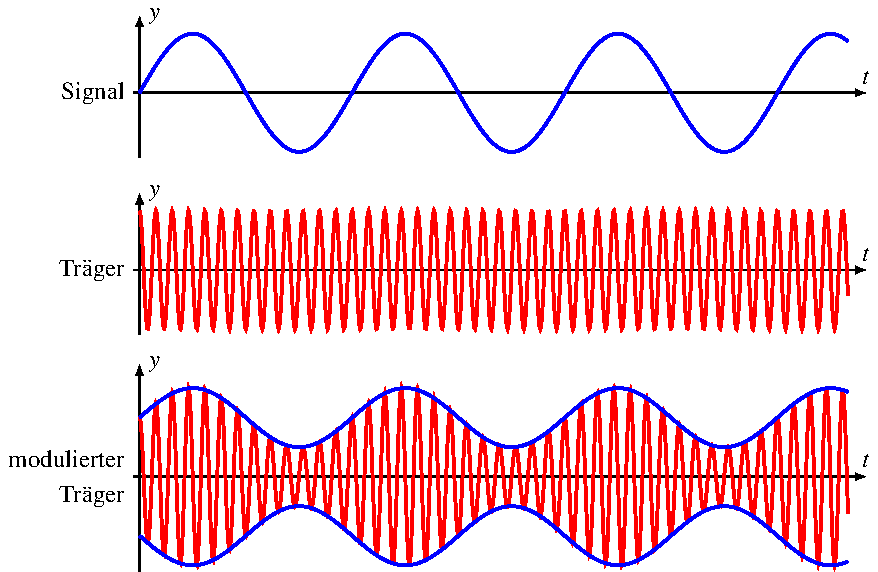
\includegraphics{applications/qam/images/am.pdf}
\caption{Amplitudenmodulation eines Signals $I(t)$ auf eine
Trägerfrequenz $\cos\omega t$.
Die Amplitude des Trägers wird im Takt des Signals verändert.
\label{figure:qam:am}}
\end{figure}

In Abbildung~\ref{figure:qam:am} wird die Amplitude des Träger
$\cos\omega t$ mit der Kreisfrequenz $\omega$ wird im Takt des
Signals verändert,
konkret wird der Träger mit $1+I(t)$ multipliziert,
das übermittelte Signal ist also
\begin{equation}
(1+I(t)) \cos\omega t.
\label{eqn:qam:am}
\end{equation}
Ein so moduliertes Signal ist besonders leicht zu demodulieren.
Es reicht, das Signal gleichzurichten und die verbleibenden Reste
der Trägerfrequenz sowie die konstente Komponten auszufiltern.
\begin{figure}
\centering
\begin{tikzpicture}
\node at (0,0) {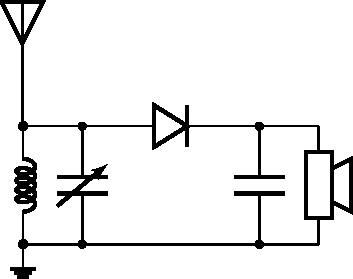
\includegraphics{applications/qam/images/detektor.pdf}};
\node at (8,0) {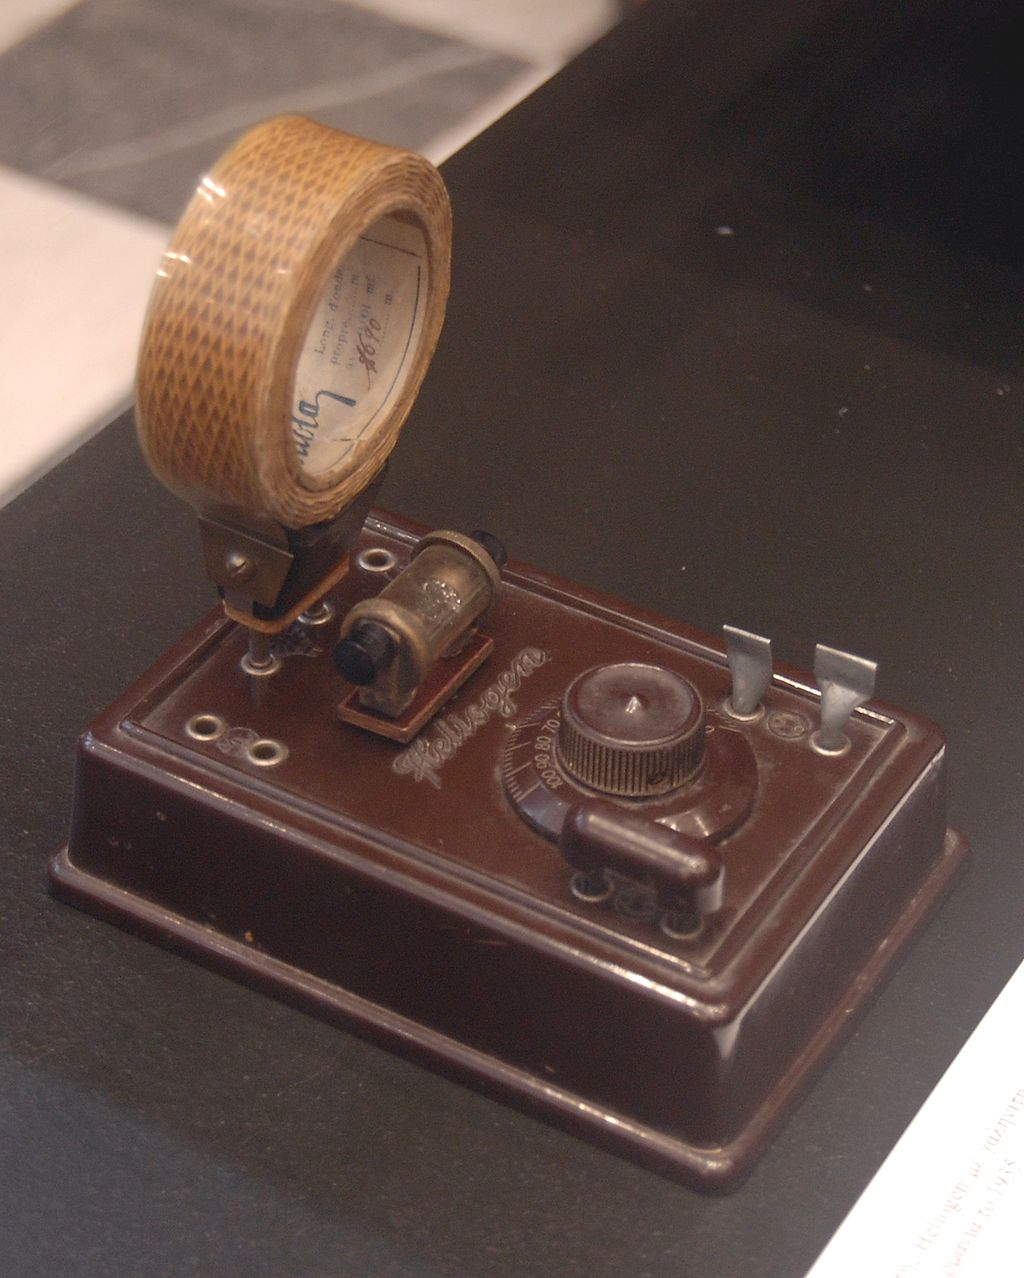
\includegraphics[width=6cm]{applications/qam/detektor.jpg}};
\end{tikzpicture}
\caption{Ein Detektorradio besteht aus einem einstellbaren
Schwingkreis zur Auswahl der Trägerfrequenz, einer Diode zur
Gleichrichtung und einem Kondensator zur Filterung der Überreste
des Trägers.
Bei starken Sendern kann das niederfrequente Tonsignal ohne
Verstärkung mit einem Kopfhörer abgehört werden.
\label{figure:qam:detektor}}
\end{figure}
Die konstante Komponente (der Summand $1$ in \eqref{eqn:qam:am})
ist nicht wirklich interessant und dient nur einer leichter
verständlichen Darstellung in Abbildung~\ref{figure:qam:am},
wir werden sie in Zukunft ignorieren und nur noch das modulierte Signal
$I(t)\cos\omega t$ betrachten.

Mit dieser Methode kann man zu jeder Zeit $t$ einen einzelnen
Wert $I(t)$ übermitteln.
Für die Praxis ist das schon bei Audiosignalen oft ungenügend, man
möchte doch mindestens die beiden Stereokanäle eines qualitativ
hochwertigen Signals übertragen können.

Die zweite Schwierigkeit ist die Frage, warum wir $\cos\omega t$
dem ebenfalls möglichen Träger $\sin\omega t$ vorziehen sollen.
Die beiden unterscheiden sich nur um eine Phasenverschiebung
von $90^\circ$, die für die oben beschriebene Modulation und
Demodulation bedeutungslos ist.






